\begin{figure}[htbp]
\centering
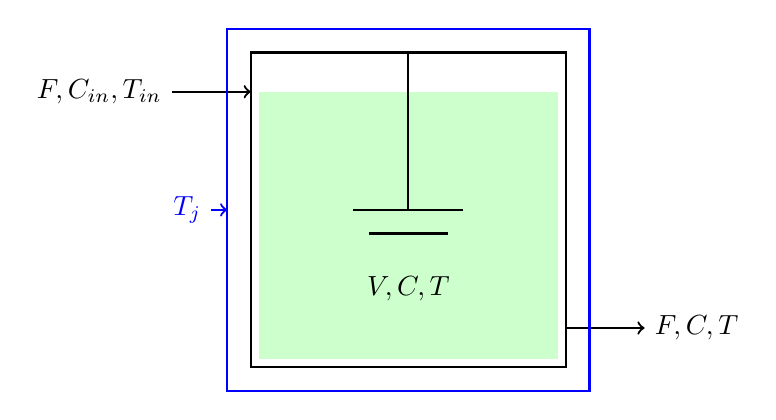
\begin{tikzpicture}
    % Tank
    \draw[thick] (0,0) -- (0,4) -- (4,4) -- (4,0) -- cycle;

    % Liquid
    \fill[green!20] (0.1,0.1) rectangle (3.9,3.5);

    % Stirrer
    \draw[thick] (2,4) -- (2,2);
    \draw[thick] (1.3,2) -- (2.7,2);
    \draw[thick] (1.5,1.7) -- (2.5,1.7);

    % Inlet
    \draw[->, thick] (-1,3.5) -- (0,3.5) node[left, pos=0] {$F, C_{\text{in}}, T_{\text{in}}$};

    % Outlet
    \draw[->, thick] (4,0.5) -- (5,0.5) node[right] {$F, C, T$};

    % Jacket
    \draw[thick, blue] (-0.3,-0.3) rectangle (4.3,4.3);
    \draw[->, thick, blue] (-0.5,2) -- (-0.3,2) node[left, pos=0] {$T_j$};

    % Labels
    \node at (2,1) {$V, C, T$};
\end{tikzpicture}
\caption{Continuous stirred-tank reactor with cooling jacket.}
\label{fig:cstr}
\end{figure}
